\documentclass[12pt]{article}
\usepackage{polski}
\usepackage{float}
\usepackage{graphicx}
\usepackage[margin=2cm]{geometry}


\title{Systemy wbudowane\\ Projekt drona}
\author{Paweł Grzegorzewski, Paweł Haraburda,  Jan Nawrat}
\date{}

\begin{document}
\maketitle

\section{Słownik pojęć}

W dokumentacji używane będą następujące pojęcia:

\begin{itemize}
    \item BSP $ - $ bezzałogowy statek powietrzny (ang. \textit{unmanned aerial vehicle, skr. UAV}), statek powietrzny bez możliwości zabierania pasażerów, w tym przypadku pilotowany zdalnie
    \item dron $ - $ inaczej BSP
    \item kontroler $ - $ niewielkie urządzenie umożliwiające sterowanie BSP na odległość poprzez RC, używające urządzenia z systemem Android lub iOS jako wyświetlacza
    \item RC $ - $ Radio Control, zdalne sterowanie realizowane drogą radiową
\end{itemize}

\section{Jakie są założenia projektu (CO)}
System zajmuje się obsługą BSP z kamerą na pokładzie, odpowiada za umożliwienie lotu oraz sterowania zewnętrzengo. Sterowanie dronem będzie odbywało się z użyciem kontrolera. Użytkownik będzie miał możliwość sterowania lotem w trzech osiach oraz zapisywania fotografii. Opcjonalnie do kontrolera będzie można podłączyć urządzenie mobilne z systemem Android lub iOS i uzyskać dostęp do poglądu z kamery pokładowej na żywo. W przypadku awarii lub utraty połączenia z kontrolerem dron podejmie próbę powrotu do miejsca startu. Wstępna kalibracja BSP będzie możliwa do wykonania przez użytkownika bez kwalifikacji ani wcześniejszego doświadczenia.

\section{W jaki sposób założenia zostaną zrealizowane (JAK)}
\begin{enumerate}
    \item Łączność modułu sterującego z BSP $ - $ dron zostanie wyposażony w moduł RC, za pomocą którego będzie łączył się z kontrolerem. Poprzez użycie połączenia USB z kontrolerem i dedykowanej aplikacji obraz z kamery na pokładzie będzie mógł być odbierany i wyświetlany na urządzeniu mobilnym.
    \item Sterowanie $ - $ kontroler będzie umożliwiał sterowanie BSP w trzech osiach poprzez odpowiednie manipulowanie dwoma drążkami (jeden w osiach x i z, drugi w osi y). Ruchy te będą odpowiednio interpretowane poprzez oprogramowanie na pokładzie drona i wysyłane będą sygnały sterujące do odpowiednich silników i powierzchni sterowych drona.
    \item Wspomaganie lotu $ - $ dron będzie wyposażony w system stabilizacji lotu, który wykorzystuje algorytmy kontroli lotu i czujniki inercyjne, zapewniając płynne i precyzyjne manewry.
    \item Podgląd na żywo $ - $ system będzie umożliwiał transmisję obrazu z kamery zainstalowanej na pokładzie drona do dedykowanej aplikacji  w czasie rzeczywistym.
    \item Wykonywanie fotografii $ - $ możliwe będzie wykonanie fotografii zintegrowaną kamerą na pokładzie drona. Kontroler będzie wyposażony w dwa przyciski oraz lampkę kontrolną przeznaczone do obsługi tej funkcji.
    \item Zapisywanie lokalizacji startowej $ - $ BSP będzie zapisywał lokalizację miejsca startowego w pamięci wewnętrznej poprzez wykorzystanie systeu GPS, co pozwali na szybkie odnalezienie punktu startowego w przypadku konieczności powrotu.
    \item Automatyczne powracanie do lokalizacji startowej $ - $ w przypadku utracenia połączenia z kontrolerem BSP automatycznie powróci do miejsca startowego wykorzystując odpowiednie algorytmy nawigacyjne i zapisaną lokalizację startową.
    \item Kalibracja przez użytkownika $ - $ procedura kalibracji BSP będzie intuicyjna i będzie możliwa do przeprowadzenia przez użytkownika bez żadnych kwalifikacji. Razem z dronem dostarczana będzie instrukcja kalibracji "krok po kroku".
    \item Diody kontrolne - każde ramię z silnikiem zostanie wyposażone w diodę kontrolną. Diody te będą ułatwiały proces kalibracji, a podczas lotu będą zwiększały widoczność BSP
\end{enumerate}
\section{Gdzie system jest wykorzystywany (GDZIE)}
Korzystać z systemu można w obszarach zamkniętych jak i otwartych. Między innymi: obszary zurbanizowane, terenty wiejskie, obszary leśne oraz górskie. Urządzenie nie nadaje się do korzystania w wodzie. 

\subsection{Ograniczenia systemu.}
Korzystając z urządzenia trzeba brać pod uwagę czynniki takie jak: 
\begin{itemize}
    \item Pogoda $-$ przy dużym wietrze mogą wystąpić problemy ze sterownością, przy wzmożonym deszczu może dojść do zwarć w systemie, bądź w momencie burz do uderzenia piorunem. W sytuacji dużego zachmurzenia lub mgły obraz z kamery może być niewyraźny oraz jest możliwe utrata widoczności drona. Korzystając z urządzenia w niższuch temperaturach prawdopodobne jest szybsze wyczerpanie akumulatora. 
    \item Wysokość $-$ w momencie osiągania większych wysokości dron stanowi poważniejsze zagrożenie w momencie awarii systemu. Trzeba też brać pod uwagę możliwe kolizje z innymi statkami powietrznymi (innymi dronami, samolotami, helikopterami).
    \item Zasięg $-$ dron posiada ograniczony zasięg latania spowodowany utratą sygnału z kontrolerem na dalszych odległościach.
    \item Prawne $-$ każde państwo posiada własne regulacje prawne dotyczące latania dronami oraz innymi bezzałogowymi statkami powietrznymi takie jak limit wysokości latania, brak możliwości latania w miastach bądź nad tłumami.
\end{itemize}

\section{Dla kogo system jest przeznaczony (KTO)}
\begin{itemize}
    \item Serwisant $-$ naprawa urządzenia, wymiana części, testowanie działania systemu.
    \item Użytkownik $-$ rekreacyjne/ekstremalne latanie dronem, robienie zdjęć/filmów, kalibracja oraz ładowanie urządzenia, podgląd z kamery urządzenia na telefonie za pomocą dedykowanej aplikacji.  
\end{itemize}



\section{Przypadki uzycia}

\begin{table}[H]
    \centering
    \begin{tabular}{|p{5cm}|p{5cm}|p{5cm}|}
    \hline
    \textbf{Nazwa PU:} Włączenie drona & \textbf{Numer PU:} 1 & \textbf{Priorytet:} wysoki \\
    \hline
    \textbf{Aktor podstawowy:} użytkownik & \multicolumn{2}{|c|}{\textbf{Typ opisu:} Ogólny}  \\
    \hline
    \multicolumn{3}{|c|}{\textbf{Udziałowcy i cele:} Użytkownik, potrzeba przełączenia switcha z off na on na dronie}\\
    \hline
    \textbf{Wyzwalacz: } Przełączenie switcha z off na on w dronie & \multicolumn{2}{|c|}{\textbf{Typ wyzwalacza:} zewnętrzny} \\
    \hline
    \multicolumn{3}{|c|}{
        \textbf{Powiązania:} Wysyłanie video live z kamery w dronie do kontrolera
    }\\
    \hline
    \multicolumn{3}{|c|}{\textbf{Zwykły przepływ zdarzeń:}
    \begin{minipage}[t]{0.6\linewidth}
        \begin{enumerate}
            \item Przesunięcię switcha z pozycji 'off' na pozycje 'on'
            \item Próba sparowania drona z kontrolerem
            \item Uruchomienie drona, pojawienie się kontrolki na dronie świadczącej o włączeniu
            \newline
        \end{enumerate}
    \end{minipage}}\\
    \hline
    \multicolumn{3}{|c|}{\textbf{Przepływy poboczne: brak}}\\
    \hline
    \multicolumn{3}{|c|}{\textbf{Przepływy alternatywne/wyjątkowe:}
    \begin{minipage}[t]{0.6\linewidth}
        \begin{enumerate}
            \item Przesunięcię switcha z pozycji 'off' na pozycje 'on'
            \item Nie włączenie się drona, spowodowane uszkodzeniem akumulatorów bądź brakiem ich naładowania 
            \newline
        \end{enumerate}
    \end{minipage}}\\
    \hline
    \end{tabular}
    \caption{Przypadki użycia dla włączenia drona}
    \label{tab:tabela_pu}
    \end{table}

\begin{table}[H]
    \centering
    \begin{tabular}{|p{5cm}|p{5cm}|p{5cm}|}
    \hline
    \textbf{Nazwa PU:} Wyłączenie drona & \textbf{Numer PU:} 2 & \textbf{Priorytet:} wysoki \\
    \hline
    \textbf{Aktor podstawowy:} użytkownik & \multicolumn{2}{|c|}{\textbf{Typ opisu:} Ogólny}  \\
    \hline
    \multicolumn{3}{|c|}{\textbf{Udziałowcy i cele:} Użytkownik, potrzeba przełączenia switcha z on na off na dronie}\\
    \hline
    \textbf{Wyzwalacz: } Przełączenie switcha z on na off w dronie & \multicolumn{2}{|c|}{\textbf{Typ wyzwalacza:} zewnętrzny} \\
    \hline
    \multicolumn{3}{|c|}{
        \textbf{Powiązania:} brak
    }\\
    \hline
    \multicolumn{3}{|c|}{\textbf{Zwykły przepływ zdarzeń:}
    \begin{minipage}[t]{0.6\linewidth}
        \begin{enumerate}
            \item Przesunięcię switcha z pozycji 'on' na pozycje 'off'
            \item Dron kończy komunikację z kontrolerem
            \item Wyłączenie drona, zniknięcie kontrolki na dronie świadczącej o włączeniu
            \newline
        \end{enumerate}
    \end{minipage}}\\
    \hline
    \multicolumn{3}{|c|}{\textbf{Przepływy poboczne: brak}}\\
    \hline
    \multicolumn{3}{|c|}{\textbf{Przepływy alternatywne/wyjątkowe:}
    \begin{minipage}[t]{0.6\linewidth}
        \begin{enumerate}
            \item Przesunięcię switcha z pozycji 'on' na pozycje 'off'
            \item Nie wyłączenie się drona, spowodowane uszkodzeniem systemu 
            \newline
        \end{enumerate}
    \end{minipage}}\\
    \hline
    \end{tabular}
    \caption{Przypadki użycia dla wyłączenia drona}
    \label{tab:tabela_pu}
    \end{table}

\begin{table}[H]
    \centering
    \begin{tabular}{|p{5cm}|p{5cm}|p{5cm}|}
    \hline
    \textbf{Nazwa PU:} Włączenie kontrolera & \textbf{Numer PU:} 3 & \textbf{Priorytet:} wysoki \\
    \hline
    \textbf{Aktor podstawowy:} użytkownik & \multicolumn{2}{|c|}{\textbf{Typ opisu:} Ogólny}  \\
    \hline
    \multicolumn{3}{|c|}{\textbf{Udziałowcy i cele:} Użytkownik, potrzeba przełączenia switcha z off na on na kontrolerze}\\
    \hline
    \textbf{Wyzwalacz: } Przełączenie switcha z 'off' na 'on' na kontrolerze & \multicolumn{2}{|c|}{\textbf{Typ wyzwalacza:} zewnętrzny} \\
    \hline
    \multicolumn{3}{|c|}{
        \textbf{Powiązania:} brak
    }\\
    \hline
    \multicolumn{3}{|c|}{\textbf{Zwykły przepływ zdarzeń:}
    \begin{minipage}[t]{0.6\linewidth}
        \begin{enumerate}
            \item Przesunięcię switcha z pozycji 'off' na pozycje 'on'
            \item Próba połączenia kontrolera z dronem
            \item Uruchomienie kontrolera, pojawienie się kontrolki na kontrolerze świadczącej o włączeniu
            \newline
        \end{enumerate}
    \end{minipage}}\\
    \hline
    \multicolumn{3}{|c|}{\textbf{Przepływy poboczne: brak}}\\
    \hline
    \multicolumn{3}{|c|}{\textbf{Przepływy alternatywne/wyjątkowe:}
    \begin{minipage}[t]{0.6\linewidth}
        \begin{enumerate}
            \item Przesunięcię switcha z pozycji 'off' na pozycje 'on'
            \item Nie włączenie się kontrolera, spowodowane uszkodzeniem akumulatorów bądź brakiem ich naładowania 
            \newline
        \end{enumerate}
    \end{minipage}}\\
    \hline
    \end{tabular}
    \caption{Przypadki użycia dla włączenia kontrolera}
    \label{tab:tabela_pu}
    \end{table}

\begin{table}[H]
    \centering
    \begin{tabular}{|p{5cm}|p{5cm}|p{5cm}|}
    \hline
    \textbf{Nazwa PU:} Wyłączenie kontrolera & \textbf{Numer PU:} 4 & \textbf{Priorytet:} wysoki \\
    \hline
    \textbf{Aktor podstawowy:} użytkownik & \multicolumn{2}{|c|}{\textbf{Typ opisu:} Ogólny}  \\
    \hline
    \multicolumn{3}{|c|}{\textbf{Udziałowcy i cele:} Użytkownik, potrzeba przełączenia switcha z 'off' na 'on' na kontrolerze}\\
    \hline
    \textbf{Wyzwalacz: } Przełączenie switcha z 'on' na 'off' na kontrolerze & \multicolumn{2}{|c|}{\textbf{Typ wyzwalacza:} zewnętrzny} \\
    \hline
    \multicolumn{3}{|c|}{
        \textbf{Powiązania:} brak
    }\\
    \hline
    \multicolumn{3}{|c|}{\textbf{Zwykły przepływ zdarzeń:}
    \begin{minipage}[t]{0.6\linewidth}
        \begin{enumerate}
            \item Przesunięcię switcha z pozycji 'on' na pozycje 'off'
            \item Zakończenie komunikacji z kontrolera z dronem
            \item Wyłączenie akumulatora
            \newline
        \end{enumerate}
    \end{minipage}}\\
    \hline
    \multicolumn{3}{|c|}{\textbf{Przepływy poboczne: brak}}\\
    \hline
    \multicolumn{3}{|c|}{\textbf{Przepływy alternatywne/wyjątkowe:}
    \begin{minipage}[t]{0.6\linewidth}
        \begin{enumerate}
            \item Przesunięcię switcha z pozycji 'off' na pozycje 'on'
            \item Nie wyłączenie się kontrolera, spowodowane uszkodzeniem systemu 
            \newline
        \end{enumerate}
    \end{minipage}}\\
    \hline
    \end{tabular}
    \caption{Przypadki użycia dla wyłączenia kontrolera}
    \label{tab:tabela_pu}
    \end{table}

\begin{table}[H]
    \centering
    \begin{tabular}{|p{5cm}|p{5cm}|p{5cm}|}
    \hline
    \textbf{Nazwa PU:} Uruchomienie silników drona & \textbf{Numer PU:} 5 & \textbf{Priorytet:} wysoki \\
    \hline
    \textbf{Aktor podstawowy:} użytkownik & \multicolumn{2}{|c|}{\textbf{Typ opisu:} szczegółowy}  \\
    \hline
    \multicolumn{3}{|c|}{\textbf{Udziałowcy i cele:} Użytkownik, potrzeba naciśnięcia przycisku na kontrolerze}\\
    \hline
    \textbf{Wyzwalacz: } Przytrzymanie przycisku 'uruchom silniki' przez 3 sekundy & \multicolumn{2}{|c|}{\textbf{Typ wyzwalacza:} zewnętrzny} \\
    \hline
    \multicolumn{3}{|c|}{
        \textbf{Powiązania:} Przesył kontroler - dron
    }\\
    \hline
    \multicolumn{3}{|c|}{\textbf{Zwykły przepływ zdarzeń:}
    \begin{minipage}[t]{0.6\linewidth}
        \begin{enumerate}
            \item Przytrzymanie przycisku 'uruchomienie silników' przez 3 sekundy
            \item Przesłanie sygnału z kontrolera do drona
            \item Dron zapisuje lokalizacje GPS
            \item Dron sprawdza czy możliwe jest włączenie silników
            \item Dron uruchamia silniki
            \newline
        \end{enumerate}
    \end{minipage}}\\
    \hline
    \multicolumn{3}{|c|}{\textbf{Przepływy poboczne: brak}}\\
    \hline
    \multicolumn{3}{|c|}{\textbf{Przepływy alternatywne/wyjątkowe:}
    \begin{minipage}[t]{0.6\linewidth}
        \begin{enumerate}
            \item Przytrzymanie przycisku 'uruchomienie silników' przez 3 sekundy
            \item Dron nie uruchamia silników z powodu braku połączenia między kontrolerem a dronem
            \item Dron nie uruchamia silników z powodu nie włączenia go 
            \newline
        \end{enumerate}
    \end{minipage}}\\
    \hline
    \end{tabular}
    \caption{Przypadki użycia dla uruchomienia silników drona}
    \label{tab:tabela_pu}
    \end{table}

\begin{table}[H]
    \centering
    \begin{tabular}{|p{5cm}|p{5cm}|p{5cm}|}
    \hline
    \textbf{Nazwa PU:} Wyłączenie silników drona & \textbf{Numer PU:} 6 & \textbf{Priorytet:} wysoki \\
    \hline
    \textbf{Aktor podstawowy:} użytkownik & \multicolumn{2}{|c|}{\textbf{Typ opisu:} szczegółowy}  \\
    \hline
    \multicolumn{3}{|c|}{\textbf{Udziałowcy i cele:} Użytkownik, potrzeba naciśnięcia przycisku na kontrolerze}\\
    \hline
    \textbf{Wyzwalacz: } Przytrzymanie przycisku 'wyłącz silniki' przez 3 sekundy & \multicolumn{2}{|c|}{\textbf{Typ wyzwalacza:} zewnętrzny} \\
    \hline
    \multicolumn{3}{|c|}{
        \textbf{Powiązania:} Przesył kontroler - dron

    }\\
    \hline
    \multicolumn{3}{|c|}{\textbf{Zwykły przepływ zdarzeń:}
    \begin{minipage}[t]{0.6\linewidth}
        \begin{enumerate}
            \item Przytrzymanie przycisku 'wyłącz silnik' przez 3 sekundy
            \item Przesłanie sygnału z kontrolera do drona
            \item Dron wyłącza silniki
            \newline
        \end{enumerate}
    \end{minipage}}\\
    \hline
    \multicolumn{3}{|c|}{\textbf{Przepływy poboczne: brak}}\\
    \hline
    \multicolumn{3}{|c|}{\textbf{Przepływy alternatywne/wyjątkowe:}
    \begin{minipage}[t]{0.6\linewidth}
        \begin{enumerate}
            \item Przytrzymanie przycisku 'wyłącz silniki' przez 3 sekundy
            \item Dron nie wyłącza silników z powodu braku połączenia między kontrolerem a dronem
            \newline
        \end{enumerate}
    \end{minipage}}\\
    \hline
    \end{tabular}
    \caption{Przypadki użycia dla wyłączenia silników drona}
    \label{tab:tabela_pu}
    \end{table}





\begin{table}[H]
\centering
\begin{tabular}{|p{5cm}|p{5cm}|p{5cm}|}
\hline
\textbf{Nazwa PU:} Wyciągnięcie karty pamięci SD & \textbf{Numer PU:} 10 & \textbf{Priorytet:} niski \\
\hline
\textbf{Aktor podstawowy:} użytkownik & \multicolumn{2}{|c|}{\textbf{Typ opisu:} ogólny} \\
\hline
\multicolumn{3}{|c|}{\textbf{Udziałowcy i cele:} Użytkownik, dron w celu przekazania karty z drona do użytkownika}\\
\hline
\textbf{Wyzwalacz: } wciśniecie płytki zawierającej karte SD & \multicolumn{2}{|c|}{\textbf{Typ wyzwalacza:} zewnętrzny} \\
\hline
\multicolumn{3}{|c|}{
    \textbf{Powiązania:} brak
}\\
\hline
\multicolumn{3}{|c|}{\textbf{Zwykły przepływ zdarzeń:}
\begin{minipage}[t]{0.6\linewidth}
    \begin{enumerate}
        \item wciśnięcie płytki zawierającej karte SD
        \item wysunięcie płytki
        \item usunięcie możliwości zapisu na karte SD w tym fotografowanie
        \item wsunięcie płytki z powrotem (poprzez użytkownika)
        \item jeśli wykryto karte to przwrócenie możliwości zapisu na karte SD
        \newline
    \end{enumerate}
\end{minipage}}\\
\hline
\multicolumn{3}{|c|}{\textbf{Przepływy poboczne: brak}}\\
\hline
\multicolumn{3}{|c|}{\textbf{Przepływy alternatywne/wyjątkowe:}
\begin{minipage}[t]{0.6\linewidth}
    \begin{enumerate}
        \item wciśnięcie płytki zawierającej karte SD
        \item nie nastpąpiło wysunięcie płytki
        \item dostęp do karty SD poprzeze rozkręcenie drona
        \item usunięcie możliwości zapisu na karte SD w tym fotografowanie
        \item skręcenie drona spowrotem (poprzez użytkownika)
        \item jeśli wykryto karte to przwrócenie możliwości zapisu na karte SD
        \newline
    \end{enumerate}
\end{minipage}}\\
\hline
\end{tabular}
\caption{Przypadki użycia dla wyciągnięcia karty pamięci SD}
\label{tab:tabela_pu}
\end{table}


\begin{table}[H]
\centering
\begin{tabular}{|p{5cm}|p{5cm}|p{5cm}|}
\hline
\textbf{Nazwa PU:} Kalibracja drona & \textbf{Numer PU:} 11 & \textbf{Priorytet:} średni \\
\hline
\textbf{Aktor podstawowy:} użytkownik & \multicolumn{2}{|c|}{\textbf{Typ opisu:} ogólny} \\
\hline
\multicolumn{3}{|c|}{\textbf{Udziałowcy i cele:} Użytkownik, dron}\\
\hline
\textbf{Wyzwalacz: Wciśnięcie przycisku służacego do kalibracji na dronie} & \multicolumn{2}{|c|}{\textbf{Typ wyzwalacza:} zewnętrzny} \\
\hline
\textbf{Powiązania:} brak\\
\hline
\multicolumn{3}{|c|}{\textbf{Zwykły przepływ zdarzeń:}
\begin{minipage}[t]{0.6\linewidth}
    \begin{enumerate}
        \item wciśnięcie przycisku rozpoczynającego kalibracje trzymając go prosto, poziomo
        \item zaświecenie się lampki kontrolnej na zielono
        \item obrócenie drona względem osi $z$ o $90\%$
        \item zaświecenie się lampki kontrolnej na zielono
        \item obrócenie drona względem osi $z$ o $90\%$
        \item zaświecenie się lampki kontrolnej na zielono
        \item obrócenie drona względem osi $z$ o $90\%$
        \item zaświecenie się lampki kontrolnej na zielono
        \item obrócenie drona względem osi $z$ o $90\%$
        \item zaświecenie się lampki kontrolnej na zielono
        \item powrót do punktu 3 tym razem względem osi $x$, kontynuacja do punktu 10, po czym powtórzenie względem osi $y$
        \item zakończenie kalibracji
        \item testowanie lotu poprzez użytkownika, jeśli efekt nie zadowalający powrót do punktu pierwszego \newline
        
    \end{enumerate}
\end{minipage}}
\\
\hline
\multicolumn{3}{|c|}{\textbf{Przepływy poboczne: brak}}\\
\hline
\multicolumn{3}{|c|}{\textbf{Przepływy alternatywne/wyjątkowe:}
\begin{minipage}[t]{0.6\linewidth}
    \begin{enumerate}
        \item wciśnięcie przycisku rozpoczynającego kalibracje        
        \item nieudana kalibracja
        \item zaświecenie się kontrolek na czerwono
        \item wyłączenie trybu kalibracji
        \newline
    \end{enumerate}
\end{minipage}}\\
\hline
\end{tabular}
\caption{Przypadki użycia dla wyciągnięcia karty pamięci SD}
\label{tab:tabela_pu}
\end{table}


\begin{table}[H]
\centering
\begin{tabular}{|p{5cm}|p{5cm}|p{5cm}|}
\hline
\textbf{Nazwa PU: }Ładowanie akumulatorów drona  & \textbf{Numer PU:} 14 & \textbf{Priorytet:} średni \\
\hline
\textbf{Aktor podstawowy:} użytkownik & \multicolumn{2}{|c|}{\textbf{Typ opisu:} ogólny} \\
\hline
\multicolumn{3}{|c|}{\textbf{Udziałowcy i cele:} Użytkownik, dron w celu naładowania akumulatorów drona}\\
\hline
\textbf{Wyzwalacz: } podpięcie kabla USB-C (podłączonego do zasilania) do drona & \multicolumn{2}{|c|}{\textbf{Typ wyzwalacza:} zewnętrzny} \\
\hline
\multicolumn{3}{|c|}{
\begin{minipage}[t]{0.6\linewidth}
    \begin{itemize}
    \item \textbf{Powiązania:} brak
    \item \textbf{Asocjacja:} brak
    \item \textbf{Zawieranie:} brak
    \item \textbf{Rozszerzenie:} brak
    \item \textbf{Generalizacja:} brak
    \end{itemize}
\end{minipage}}\\
\hline
\multicolumn{3}{|c|}{\textbf{Zwykły przepływ zdarzeń:}
\begin{minipage}[t]{0.6\linewidth}
    \begin{enumerate}
        \item podpięcie kabla USB-C (podłączonego do zasilania) do drona
        \item rozpoczęcie procesu ładowania akumulatorów
        \item osięgniecie maskymalnej pojemnośći akumulatorów
        \item wyciągneicie kabla zasilającego
        \newline
    \end{enumerate}
\end{minipage}}\\
\hline
\multicolumn{3}{|c|}{\textbf{Przepływy poboczne:}
\begin{minipage}[t]{0.6\linewidth}
    \begin{enumerate}
        \item podpięcie kabla USB-C (podłączonego do zasilania) do drona
        \item rozpoczęcie procesu ładowania akumulatorów
        \item wyciągneicie kabla zasilającego
        \newline
    \end{enumerate}
\end{minipage}}\\
\hline
\multicolumn{3}{|c|}{\textbf{Przepływy alternatywne/wyjątkowe:} brak}\\
\hline
\end{tabular}
\caption{Przypadki użycia dla ładowania drona }
\label{tab:tabela_pu}
\end{table}



\begin{table}[H]
\centering
\begin{tabular}{|p{5cm}|p{5cm}|p{5cm}|}
\hline
\textbf{Nazwa PU: }Ładowanie akumulatorów kontrolera  & \textbf{Numer PU:} 15 & \textbf{Priorytet:} średni \\
\hline
\textbf{Aktor podstawowy:} użytkownik & \multicolumn{2}{|c|}{\textbf{Typ opisu:} ogólny} \\
\hline
\multicolumn{3}{|c|}{\textbf{Udziałowcy i cele:} Użytkownik, kontroler w celu naładowania akumulatorów kontrolera}\\
\hline
\textbf{Wyzwalacz: } podpięcie kabla USB-C (podłączonego do zasilania) do kontrolera & \multicolumn{2}{|c|}{\textbf{Typ wyzwalacza:} zewnętrzny} \\
\hline
\multicolumn{3}{|c|}{
\begin{minipage}[t]{0.6\linewidth}
    \begin{itemize}
    \item \textbf{Powiązania:} brak
    \item \textbf{Asocjacja:} brak
    \item \textbf{Zawieranie:} brak
    \item \textbf{Rozszerzenie:} brak
    \item \textbf{Generalizacja:} brak
    \end{itemize}
\end{minipage}}\\
\hline
\multicolumn{3}{|c|}{\textbf{Zwykły przepływ zdarzeń:}
\begin{minipage}[t]{0.6\linewidth}
    \begin{enumerate}
        \item podpięcie kabla USB-C (podłączonego do zasilania) do kontrolera
        \item rozpoczęcie procesu ładowania akumulatorów
        \item osięgniecie maskymalnej pojemnośći akumulatorów
        \item wyciągneicie kabla zasilającego
        \newline
    \end{enumerate}
\end{minipage}}\\
\hline
\multicolumn{3}{|c|}{\textbf{Przepływy poboczne:}
\begin{minipage}[t]{0.6\linewidth}
    \begin{enumerate}
        \item podpięcie kabla USB-C (podłączonego do zasilania) do kontrolera
        \item rozpoczęcie procesu ładowania akumulatorów
        \item wyciągneicie kabla zasilającego
        \newline
    \end{enumerate}
\end{minipage}}\\
\hline
\multicolumn{3}{|c|}{\textbf{Przepływy alternatywne/wyjątkowe:} brak}\\
\hline
\end{tabular}
\caption{Przypadki użycia dla ładowania kontrolera }
\label{tab:tabela_pu}
\end{table}


\begin{table}[H]
\centering
\begin{tabular}{|p{5cm}|p{5cm}|p{5cm}|}
\hline
\textbf{Nazwa PU: }Wysyłanie obrazu z kamery na żywo  & \textbf{Numer PU:} 16 & \textbf{Priorytet:} średni \\
\hline
\textbf{Aktor podstawowy:} dron & \multicolumn{2}{|c|}{\textbf{Typ opisu:} szczegółowy} \\
\hline
\multicolumn{3}{|c|}{\textbf{Udziałowcy i cele:} dron oraz kontroler z podłaczonym telefonem w celu udostępnienia możliwości poglądu widoku z drona na żywo}\\
\hline
\textbf{Wyzwalacz: } uruchomienie drona & \multicolumn{2}{|c|}{\textbf{Typ wyzwalacza:} zewnętrzny} \\
\hline
\multicolumn{3}{|c|}{
\begin{minipage}[t]{0.6\linewidth}
    \begin{itemize}
    \item \textbf{Powiązania:} Podłączenie telefonu do kontrolera
    \item \textbf{Asocjacja:} brak
    \item \textbf{Zawieranie:} brak
    \item \textbf{Rozszerzenie:} brak
    \item \textbf{Generalizacja:} brak
    \end{itemize}
\end{minipage}}\\
\hline
\multicolumn{3}{|c|}{\textbf{Zwykły przepływ zdarzeń:}
\begin{minipage}[t]{0.6\linewidth}
    \begin{enumerate}
        \item włączenie drona
        \item uruchomienie kamery
        \item rozpoczęcie przesyłu wideo
        \item odbiór wideo poprzez kontroler
        \item przesłane wideo do podłączonego urządzenia mobilnego
        \item wyświetlenie wideo poprzeez podłaczone urządzenie
        \newline
    \end{enumerate}
\end{minipage}}\\
\hline
\multicolumn{3}{|c|}{\textbf{Przepływy poboczne:} \begin{minipage}[t]{0.6\linewidth}
    \begin{enumerate}
        \item włączenie drona
        \item rozpoczęcie wysyłania wideo
        \item odbiór wideo poprzez kontroler
        \item nie wykryto podłaczonego urządzenia mobilnego
        \item oczekiwanie w tle, kontrolera na podłączenie telefonu
        \item przejście do przypadku użycia "Podłączenie telefonu do kontrolera"
        \newline
    \end{enumerate}
\end{minipage}}
\\
\hline
\multicolumn{3}{|c|}{\textbf{Przepływy alternatywne/wyjątkowe:} brak}\\
\hline
\end{tabular}
\caption{Przypadki użycia dla przesyłania obrazu na żywo }
\label{tab:tabela_pu}
\end{table}






\begin{table}[H]
\centering
\begin{tabular}{|p{5cm}|p{5cm}|p{5cm}|}
\hline
\textbf{Nazwa PU: } Wykonanie ruchu  & \textbf{Numer PU:} 17 & \textbf{Priorytet:} wysoki \\
\hline
\textbf{Aktor podstawowy:} użytkownik & \multicolumn{2}{|c|}{\textbf{Typ opisu:} szczegółowy} \\
\hline
\multicolumn{3}{|c|}{\textbf{Udziałowcy i cele:} użytkownik, kontroler, dron}\\
\hline
\textbf{Wyzwalacz: } zmiana pozycji jednego lub więcej z drążków kontrolera & \multicolumn{2}{|c|}{\textbf{Typ wyzwalacza:} zewnętrzny} \\
\hline
\multicolumn{3}{|c|}{
\begin{minipage}[t]{0.6\linewidth}
    \begin{itemize}
    \item \textbf{Powiązania:} brak
    \item \textbf{Asocjacja:} brak
    \item \textbf{Zawieranie:} brak
    \item \textbf{Rozszerzenie:} Wysłanie sygnału do drona
    \item \textbf{Generalizacja:} brak
    \end{itemize}
\end{minipage}}\\
\hline
\multicolumn{3}{|c|}{\textbf{Zwykły przepływ zdarzeń:}
\begin{minipage}[t]{0.6\linewidth}
    \begin{enumerate}
        \item kontroler zczytuje aktualne pozycje drążków
        \item kontroler wysyła informację o wprowadzonym ruchu do drona
        \item dron otrzymuje sygnał z informacją o ruchu
        \item na podstawie inforamcji z sensorów na pokładzie dron ustala, czy ruch zakończy się kolizją
        \item dron ustala jakie ustawienie silników poskutkuje wykonaniem ruchu po czym je wdraża
        \newline
    \end{enumerate}
\end{minipage}}\\
\hline
\multicolumn{3}{|c|}{\textbf{Przepływy poboczne:}
\begin{minipage}[t]{0.6\linewidth}
    \begin{enumerate}
        \item[1a)] kontroler zczytuje aktualne pozycje drążków
        \item[1b)] kontroler wysyła informację o wprowadzonym ruchu do drona
        \item[1c)] dron otrzymuje sygnał z informacją o ruchu
        \item[1d)] na podstawie inforamcji z sensorów na pokładzie dron ustala, czy ruch zakończy się kolizją
        \item[1e)] dron nie wykonuje ruchu, ponieważ wykrył możliwość kolizji
        \newline
    \end{enumerate}
\end{minipage}}\\
\hline
\multicolumn{3}{|c|}{\textbf{Przepływy alternatywne/wyjątkowe:} brak}\\
\hline
\end{tabular}
\caption{Przypadek użycia: Wykonanie ruchu}
\label{tab:tabela_pu}
\end{table}



\begin{table}[H]
\centering
\begin{tabular}{|p{5cm}|p{5cm}|p{5cm}|}
\hline
\textbf{Nazwa PU: } Lądowanie  & \textbf{Numer PU:} 18 & \textbf{Priorytet:} średni \\
\hline
\textbf{Aktor podstawowy:} użytkownik & \multicolumn{2}{|c|}{\textbf{Typ opisu:} szczegółowy} \\
\hline
\multicolumn{3}{|c|}{\textbf{Udziałowcy i cele:} użytkownik, kontroler, dron}\\
\hline
\textbf{Wyzwalacz: } wciśnięcie dedykowanego przycisku lądowania na kontrolerze & \multicolumn{2}{|c|}{\textbf{Typ wyzwalacza:} zewnętrzny} \\
\hline
\multicolumn{3}{|c|}{
\begin{minipage}[t]{0.6\linewidth}
    \begin{itemize}
    \item \textbf{Powiązania:} Wykonanie ruchu
    \item \textbf{Asocjacja:} brak
    \item \textbf{Zawieranie:} brak
    \item \textbf{Rozszerzenie:} Wysłanie sygnału do drona
    \item \textbf{Generalizacja:} brak
    \end{itemize}
\end{minipage}}\\
\hline
\multicolumn{3}{|c|}{\textbf{Zwykły przepływ zdarzeń:}
\begin{minipage}[t]{0.6\linewidth}
    \begin{enumerate}
        \item kontroler wysyła sygnał do drona z informacją o rządaniu lądowania
        \item dron otrzymuje sygnał
        \item dron rozpoczyna manewr lądowania wspomagając się sensorami
        \item dron kończy lądowanie gdy odczyta z sensorów, że znalazł się na podłożu
        \newline
    \end{enumerate}
\end{minipage}}\\
\hline
\multicolumn{3}{|c|}{\textbf{Przepływy poboczne:}
\begin{minipage}[t]{0.6\linewidth}
    \begin{enumerate}
        \item[1a)] kontroler wysyła sygnał do drona z informacją o rządaniu lądowania
        \item[1b)] dron otrzymuje sygnał
        \item[1c)] dron rozpoczyna manewr lądowania wspomagając się sensorami
        \item[1d)] użytkownik rozpoczął wykonywanie ruchu
        \item[1e)] dron otrzymuje sygnał z rządaniem wykonaniu ruchu i porzuca operację lądowania
        \newline
    \end{enumerate}
\end{minipage}}\\
\hline
\multicolumn{3}{|c|}{\textbf{Przepływy alternatywne/wyjątkowe:}
\begin{minipage}[t]{0.6\linewidth}
    \begin{enumerate}
        \item[1a)] kontroler wysyła sygnał do drona z informacją o rządaniu lądowania
        \item[1b)] dron otrzymuje sygnał
        \item[1c)] dron rozpoczyna manewr lądowania wspomagając się sensorami
        \item[1d)] dron wykrywa nieprzewidzianą zmianę położenia
        \item[1e)] dron stabilizuje się i porzuca wykonanie manewru lądowania
        \newline
    \end{enumerate}
\end{minipage}}\\
\hline
\end{tabular}
\caption{Przypadek użycia: Lądowanie}
\label{tab:tabela_pu}
\end{table}




\begin{table}[H]
\centering
\begin{tabular}{|p{5cm}|p{5cm}|p{5cm}|}
\hline
\textbf{Nazwa PU: } Wysyłanie sygnału PING do drona & \textbf{Numer PU:} 19 & \textbf{Priorytet:} średni \\
\hline
\textbf{Aktor podstawowy:} kontroler & \multicolumn{2}{|c|}{\textbf{Typ opisu:} szczegółowy} \\
\hline
\multicolumn{3}{|c|}{\textbf{Udziałowcy i cele:} kontroler, dron}\\
\hline
\textbf{Wyzwalacz: } przerwanie przez wewnętrzny timer & \multicolumn{2}{|c|}{\textbf{Typ wyzwalacza:} wewnętrzny} \\
\hline
\multicolumn{3}{|c|}{
\begin{minipage}[t]{0.6\linewidth}
    \begin{itemize}
    \item \textbf{Powiązania:} Powrót do miejsca startu
    \item \textbf{Asocjacja:} brak
    \item \textbf{Zawieranie:} brak
    \item \textbf{Rozszerzenie:} Wysłanie sygnału do drona
    \item \textbf{Generalizacja:} brak
    \end{itemize}
\end{minipage}}\\
\hline
\multicolumn{3}{|c|}{\textbf{Zwykły przepływ zdarzeń:}
\begin{minipage}[t]{0.6\linewidth}
    \begin{enumerate}
        \item kontroler wysyła sygnał do drona
        \item dron odbiera sygnał i zapisuje nowy czas otrzymania ostatniego sygnału
        \newline
    \end{enumerate}
\end{minipage}}\\
\hline
\multicolumn{3}{|c|}{\textbf{Przepływy poboczne:}
\begin{minipage}[t]{0.6\linewidth}
    \begin{enumerate}
        \item[1a)] kontroler wysyła sygnał do drona
        \item[1b)] sygnał nie dociera
        \newline
    \end{enumerate}
\end{minipage}}\\
\hline
\multicolumn{3}{|c|}{\textbf{Przepływy alternatywne/wyjątkowe:}}\\
\hline
\end{tabular}
\caption{Przypadek użycia: Wysyłanie sygnału PING do drona}
\label{tab:tabela_pu}
\end{table}


\begin{table}[H]
\centering
\begin{tabular}{|p{5cm}|p{5cm}|p{5cm}|}
\hline
\textbf{Nazwa PU: } Powrót do miejsca startu  & \textbf{Numer PU:} 20 & \textbf{Priorytet:} średni \\
\hline
\textbf{Aktor podstawowy:} dron & \multicolumn{2}{|c|}{\textbf{Typ opisu:} szczegółowy} \\
\hline
\multicolumn{3}{|c|}{\textbf{Udziałowcy i cele:} kontroler(w przepływie pobocznym), dron}\\
\hline
\textbf{Wyzwalacz: } przerwanie związane z nieotrzymaniem sygnału PING od kontrolera & \multicolumn{2}{|c|}{\textbf{Typ wyzwalacza:} wewnętrzny} \\
\hline
\multicolumn{3}{|c|}{
\begin{minipage}[t]{0.6\linewidth}
    \begin{itemize}
    \item \textbf{Powiązania:} Wysłanie sygnału PING do drona
    \item \textbf{Asocjacja:} Lądowanie
    \item \textbf{Zawieranie:} brak
    \item \textbf{Rozszerzenie:} Wysłanie sygnału do drona
    \item \textbf{Generalizacja:} brak
    \end{itemize}
\end{minipage}}\\
\hline
\multicolumn{3}{|c|}{\textbf{Zwykły przepływ zdarzeń:}
\begin{minipage}[t]{0.6\linewidth}
    \begin{enumerate}
        \item dron odczytuje z pamięci wewnętrznej miejsce włączenia silników
        \item dron wznosi się na odpowiednią wysokość
        \item dron odczytuje swoją aktualną lokalizację i kieruje się w miejsce startu
        \item po dotarciu do miejsca startu dron rozpoczyna procedurę lądowania
        \newline
    \end{enumerate}
\end{minipage}}\\
\hline
\multicolumn{3}{|c|}{\textbf{Przepływy poboczne:}
\begin{minipage}[t]{0.6\linewidth}
    \begin{enumerate}
        \item[1a)] w czasie wykonywania procedury powrotu dron ponownie nawiązuje sygnał z kontrolerem
        \item[1b)] dron stabilizuje pozycję i przerywa procedurę powrotu
        \newline
    \end{enumerate}
\end{minipage}}\\
\hline
\multicolumn{3}{|c|}{\textbf{Przepływy alternatywne/wyjątkowe:}
\begin{minipage}[t]{0.6\linewidth}
    \begin{enumerate}
        \item[1a)] dron odczytuje z pamięci wewnętrznej miejsce włączenia silników
        \item[1b)] dron wznosi się na odpowiednią wysokość
        \item[1c)] dron odczytuje swoją aktualną lokalizację i kieruje się w miejsce startu
        \item[1d)] dron natrafia na przeszkodę i przerywa procedurę powrotu
        \item[2a)] bateria osiąga bardzo niski poziom
        \item[2b)] dron wykonuje procedurę lądowania 
        \newline
    \end{enumerate}
\end{minipage}}\\
\hline
\end{tabular}
\caption{Przypadek użycia: Powrót do miejsca startu}
\label{tab:tabela_pu}
\end{table}



\begin{table}[H]
\centering
\begin{tabular}{|p{5cm}|p{5cm}|p{5cm}|}
\hline
\textbf{Nazwa PU: } Podłączenie telefonu do kontrolera  & \textbf{Numer PU:} 21 & \textbf{Priorytet:} niski \\
\hline
\textbf{Aktor podstawowy:} użytkownik & \multicolumn{2}{|c|}{\textbf{Typ opisu:} szczegółowy} \\
\hline
\multicolumn{3}{|c|}{\textbf{Udziałowcy i cele:} użytkownik, kontroler}\\
\hline
\textbf{Wyzwalacz: } nawiązanie połączenia USB z telefonem z systemem iOS lub Android & \multicolumn{2}{|c|}{\textbf{Typ wyzwalacza:} zewnętrzny} \\
\hline
\multicolumn{3}{|c|}{
\begin{minipage}[t]{0.6\linewidth}
    \begin{itemize}
    \item \textbf{Powiązania:} Wysyłanie wideo na żywo
    \item \textbf{Asocjacja:} brak
    \item \textbf{Zawieranie:} brak
    \item \textbf{Rozszerzenie:} brak
    \item \textbf{Generalizacja:} brak
    \end{itemize}
\end{minipage}}\\
\hline
\multicolumn{3}{|c|}{\textbf{Zwykły przepływ zdarzeń:}
\begin{minipage}[t]{0.6\linewidth}
    \begin{enumerate}
        \item kontroler czeka na uruchomienie dedykowanej aplikacji
        \item po włączeniu aplikacji obraz na żywo zaczyna być wyświetlany
        \newline
    \end{enumerate}
\end{minipage}}\\
\hline
\multicolumn{3}{|c|}{\textbf{Przepływy poboczne:}
\begin{minipage}[t]{0.6\linewidth}
    \begin{enumerate}
        \item[1a)] kontroler czeka na uruchomienie dedykowanej aplikacji
        \item[1b)] po włączeniu aplikacji obraz na żywo zaczyna być wyświetlany
        \item[1c)] obraz nie jest dostępny
        \item[1d)] na ekranie wyświetlana jest odpowiednia informacja
        \newline
    \end{enumerate}
\end{minipage}}\\
\hline
\multicolumn{3}{|c|}{\textbf{Przepływy alternatywne/wyjątkowe:}}\\
\hline
\end{tabular}
\caption{Przypadek użycia: Podłączenie telefonu do kontrolera}
\label{tab:tabela_pu}
\end{table}





\begin{table}[H]
\centering
\begin{tabular}{|p{5cm}|p{5cm}|p{5cm}|}
\hline
\textbf{Nazwa PU: } Odłączenie telefonu od kontrolera  & \textbf{Numer PU:} 22 & \textbf{Priorytet:} niski \\
\hline
\textbf{Aktor podstawowy:} użytkownik & \multicolumn{2}{|c|}{\textbf{Typ opisu:} szczegółowy} \\
\hline
\multicolumn{3}{|c|}{\textbf{Udziałowcy i cele:} użytkownik, kontroler}\\
\hline
\textbf{Wyzwalacz: } odłączenie od kontrolera telefonu & \multicolumn{2}{|c|}{\textbf{Typ wyzwalacza:} zewnętrzny} \\
\hline
\multicolumn{3}{|c|}{
\begin{minipage}[t]{0.6\linewidth}
    \begin{itemize}
    \item \textbf{Powiązania:} Wysyłanie wideo na żywo
    \item \textbf{Asocjacja:} brak
    \item \textbf{Zawieranie:} brak
    \item \textbf{Rozszerzenie:} brak
    \item \textbf{Generalizacja:} brak
    \end{itemize}
\end{minipage}}\\
\hline
\multicolumn{3}{|c|}{\textbf{Zwykły przepływ zdarzeń:}
\begin{minipage}[t]{0.6\linewidth}
    \begin{enumerate}
        \item kontroler przestaje wysyłać obraz przez port USB
        \newline
    \end{enumerate}
\end{minipage}}\\
\hline
\multicolumn{3}{|c|}{\textbf{Przepływy poboczne:}}\\
\hline
\multicolumn{3}{|c|}{\textbf{Przepływy alternatywne/wyjątkowe:}}\\
\hline
\end{tabular}
\caption{Przypadek użycia: Odłączenie telefonu od kontrolera}
\label{tab:tabela_pu}
\end{table}



\begin{table}[H]
\centering
\begin{tabular}{|p{5cm}|p{5cm}|p{5cm}|}
\hline
\textbf{Nazwa PU: } Wykonanie zdjęcia & \textbf{Numer PU:} 23 & \textbf{Priorytet:} średni \\
\hline
\textbf{Aktor podstawowy:} użytkownik & \multicolumn{2}{|c|}{\textbf{Typ opisu:} szczegółowy} \\
\hline
\multicolumn{3}{|c|}{\textbf{Udziałowcy i cele:} użytkownik, kontroler, dron}\\
\hline
\textbf{Wyzwalacz: } wciśnięcie dedykowanego przycisku na kontrolerze & \multicolumn{2}{|c|}{\textbf{Typ wyzwalacza:} zewnętrzny} \\
\hline
\multicolumn{3}{|c|}{
\begin{minipage}[t]{0.6\linewidth}
    \begin{itemize}
    \item \textbf{Powiązania, asocjacja i zawieranie} brak
    \item \textbf{Rozszerzenie:} Wysłanie sygnału do drona
    \item \textbf{Generalizacja:} brak
    \end{itemize}
\end{minipage}}\\
\hline
\multicolumn{3}{|c|}{\textbf{Zwykły przepływ zdarzeń:}
\begin{minipage}[t]{0.6\linewidth}
    \begin{enumerate}
        \item kontroler wysyła do drona sygnał z rządaniem zrobienia zdjęcia
        \item dron odbiera sygnał
        \item dron sprawdza czy dostępna jest karta SD z wystarczającą ilością wolnego miejsca
        \item dron wykonuje zdjęcia z kamery i zapisuje je na karcie SD
        \newline
    \end{enumerate}
\end{minipage}}\\
\hline
\multicolumn{3}{|c|}{\textbf{Przepływy poboczne:}
\begin{minipage}[t]{0.6\linewidth}
    \begin{enumerate}
        \item[1a)] w czasie wykonywania procedury powrotu dron ponownie nawiązuje sygnał z kontrolerem
        \item[1b)] dron stabilizuje pozycję i przerywa procedurę powrotu
        \newline
    \end{enumerate}
\end{minipage}}\\
\hline
\multicolumn{3}{|c|}{\textbf{Przepływy alternatywne/wyjątkowe:}
\begin{minipage}[t]{0.6\linewidth}
    \begin{enumerate}
        \item[1a)] kontroler wysyła do drona sygnał z rządaniem zrobienia zdjęcia
        \item[1b)] dron odbiera sygnał
        \item[1c)] dron sprawdza czy dostępna jest karta SD z wystarczającą ilością wolnego miejsca
        \item[1d)] dron nie wykrywa obecności karty SD i przerywa operację
        \item[2a)] kontroler wysyła do drona sygnał z rządaniem zrobienia zdjęcia
        \item[2b)] dron odbiera sygnał
        \item[2c)] dron sprawdza czy dostępna jest karta SD z wystarczającą ilością wolnego miejsca
        \item[2d)] na karcie SD nie ma wystarczająco wolnego miejsca i dron przerywa operację
        \newline
    \end{enumerate}
\end{minipage}}\\
\hline
\end{tabular}
\caption{Przypadek użycia: Wykonanie zdjęcia}
\label{tab:tabela_pu}
\end{table}

\newpage
\section{Diagram przypadków użycia}
\begin{figure}[h]
    \centering
    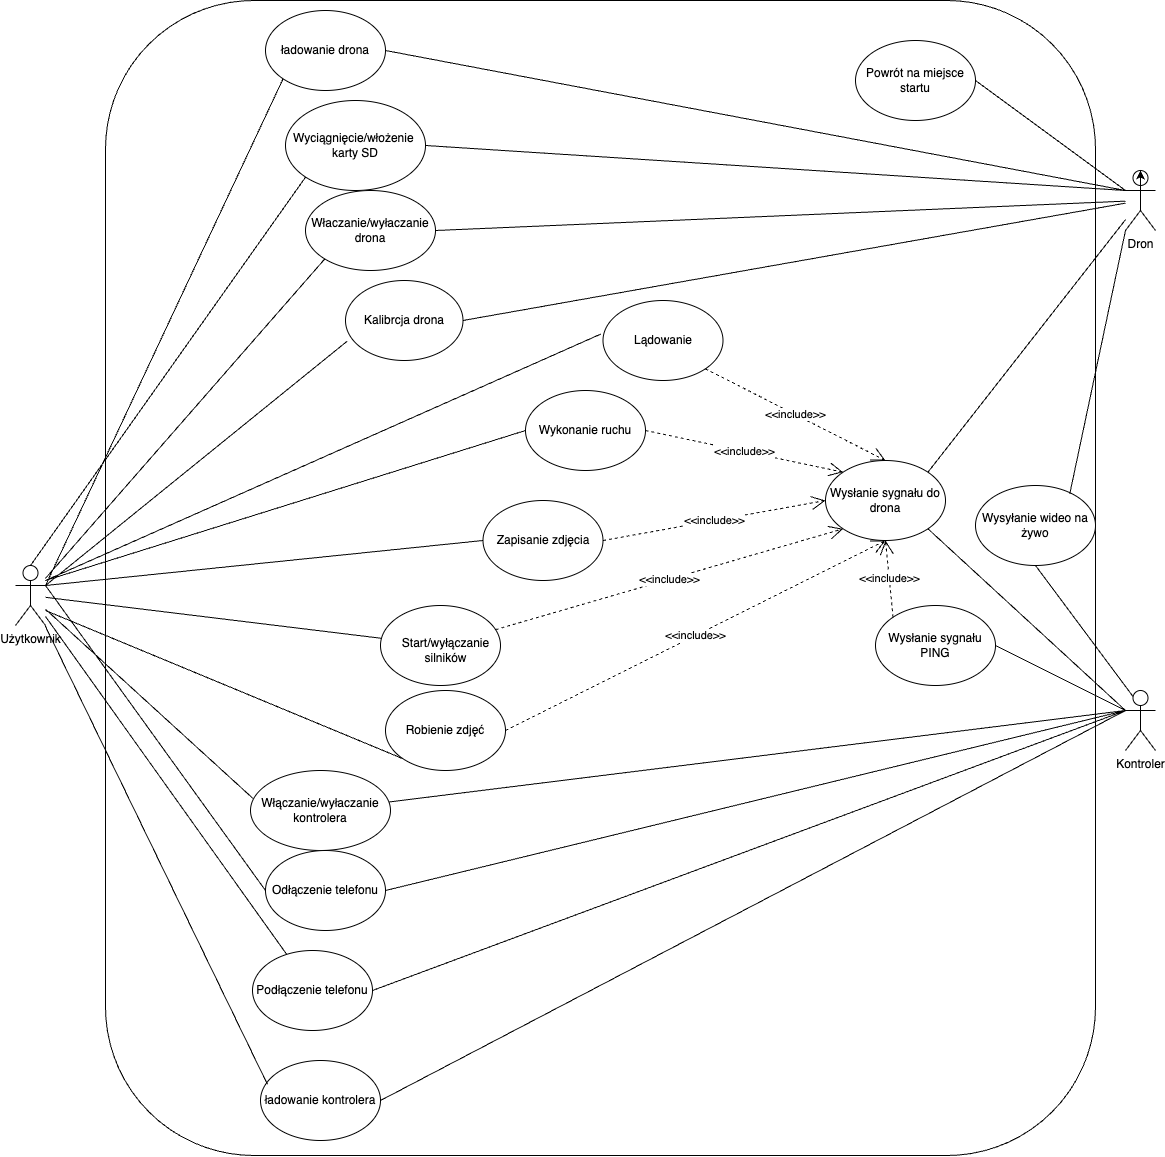
\includegraphics[width=0.95\textwidth]{../resources/diagramWbudowane.drawio.png}
    \caption{Diagram przypadków użycia}
    \label{fig:example}
\end{figure}

\end{document}
